% Options for packages loaded elsewhere
\PassOptionsToPackage{unicode}{hyperref}
\PassOptionsToPackage{hyphens}{url}
%
\documentclass[
  9 pt,
  ignorenonframetext,
]{beamer}
\usepackage{pgfpages}
\setbeamertemplate{caption}[numbered]
\setbeamertemplate{caption label separator}{: }
\setbeamercolor{caption name}{fg=normal text.fg}
\beamertemplatenavigationsymbolsempty
% Prevent slide breaks in the middle of a paragraph
\widowpenalties 1 10000
\raggedbottom
\setbeamertemplate{part page}{
  \centering
  \begin{beamercolorbox}[sep=16pt,center]{part title}
    \usebeamerfont{part title}\insertpart\par
  \end{beamercolorbox}
}
\setbeamertemplate{section page}{
  \centering
  \begin{beamercolorbox}[sep=12pt,center]{part title}
    \usebeamerfont{section title}\insertsection\par
  \end{beamercolorbox}
}
\setbeamertemplate{subsection page}{
  \centering
  \begin{beamercolorbox}[sep=8pt,center]{part title}
    \usebeamerfont{subsection title}\insertsubsection\par
  \end{beamercolorbox}
}
\AtBeginPart{
  \frame{\partpage}
}
\AtBeginSection{
  \ifbibliography
  \else
    \frame{\sectionpage}
  \fi
}
\AtBeginSubsection{
  \frame{\subsectionpage}
}
\usepackage{amsmath,amssymb}
\usepackage{lmodern}
\usepackage{ifxetex,ifluatex}
\ifnum 0\ifxetex 1\fi\ifluatex 1\fi=0 % if pdftex
  \usepackage[T1]{fontenc}
  \usepackage[utf8]{inputenc}
  \usepackage{textcomp} % provide euro and other symbols
\else % if luatex or xetex
  \usepackage{unicode-math}
  \defaultfontfeatures{Scale=MatchLowercase}
  \defaultfontfeatures[\rmfamily]{Ligatures=TeX,Scale=1}
\fi
\usetheme[]{Dresden}
\usecolortheme{seagull}
\usefonttheme{structuresmallcapsserif}
% Use upquote if available, for straight quotes in verbatim environments
\IfFileExists{upquote.sty}{\usepackage{upquote}}{}
\IfFileExists{microtype.sty}{% use microtype if available
  \usepackage[]{microtype}
  \UseMicrotypeSet[protrusion]{basicmath} % disable protrusion for tt fonts
}{}
\makeatletter
\@ifundefined{KOMAClassName}{% if non-KOMA class
  \IfFileExists{parskip.sty}{%
    \usepackage{parskip}
  }{% else
    \setlength{\parindent}{0pt}
    \setlength{\parskip}{6pt plus 2pt minus 1pt}}
}{% if KOMA class
  \KOMAoptions{parskip=half}}
\makeatother
\usepackage{xcolor}
\IfFileExists{xurl.sty}{\usepackage{xurl}}{} % add URL line breaks if available
\IfFileExists{bookmark.sty}{\usepackage{bookmark}}{\usepackage{hyperref}}
\hypersetup{
  pdftitle={Untitled},
  pdfauthor={Ana Luzielma ; Jaylhane Nunes ; Raianny Soares},
  hidelinks,
  pdfcreator={LaTeX via pandoc}}
\urlstyle{same} % disable monospaced font for URLs
\newif\ifbibliography
\usepackage{color}
\usepackage{fancyvrb}
\newcommand{\VerbBar}{|}
\newcommand{\VERB}{\Verb[commandchars=\\\{\}]}
\DefineVerbatimEnvironment{Highlighting}{Verbatim}{commandchars=\\\{\}}
% Add ',fontsize=\small' for more characters per line
\usepackage{framed}
\definecolor{shadecolor}{RGB}{248,248,248}
\newenvironment{Shaded}{\begin{snugshade}}{\end{snugshade}}
\newcommand{\AlertTok}[1]{\textcolor[rgb]{0.94,0.16,0.16}{#1}}
\newcommand{\AnnotationTok}[1]{\textcolor[rgb]{0.56,0.35,0.01}{\textbf{\textit{#1}}}}
\newcommand{\AttributeTok}[1]{\textcolor[rgb]{0.77,0.63,0.00}{#1}}
\newcommand{\BaseNTok}[1]{\textcolor[rgb]{0.00,0.00,0.81}{#1}}
\newcommand{\BuiltInTok}[1]{#1}
\newcommand{\CharTok}[1]{\textcolor[rgb]{0.31,0.60,0.02}{#1}}
\newcommand{\CommentTok}[1]{\textcolor[rgb]{0.56,0.35,0.01}{\textit{#1}}}
\newcommand{\CommentVarTok}[1]{\textcolor[rgb]{0.56,0.35,0.01}{\textbf{\textit{#1}}}}
\newcommand{\ConstantTok}[1]{\textcolor[rgb]{0.00,0.00,0.00}{#1}}
\newcommand{\ControlFlowTok}[1]{\textcolor[rgb]{0.13,0.29,0.53}{\textbf{#1}}}
\newcommand{\DataTypeTok}[1]{\textcolor[rgb]{0.13,0.29,0.53}{#1}}
\newcommand{\DecValTok}[1]{\textcolor[rgb]{0.00,0.00,0.81}{#1}}
\newcommand{\DocumentationTok}[1]{\textcolor[rgb]{0.56,0.35,0.01}{\textbf{\textit{#1}}}}
\newcommand{\ErrorTok}[1]{\textcolor[rgb]{0.64,0.00,0.00}{\textbf{#1}}}
\newcommand{\ExtensionTok}[1]{#1}
\newcommand{\FloatTok}[1]{\textcolor[rgb]{0.00,0.00,0.81}{#1}}
\newcommand{\FunctionTok}[1]{\textcolor[rgb]{0.00,0.00,0.00}{#1}}
\newcommand{\ImportTok}[1]{#1}
\newcommand{\InformationTok}[1]{\textcolor[rgb]{0.56,0.35,0.01}{\textbf{\textit{#1}}}}
\newcommand{\KeywordTok}[1]{\textcolor[rgb]{0.13,0.29,0.53}{\textbf{#1}}}
\newcommand{\NormalTok}[1]{#1}
\newcommand{\OperatorTok}[1]{\textcolor[rgb]{0.81,0.36,0.00}{\textbf{#1}}}
\newcommand{\OtherTok}[1]{\textcolor[rgb]{0.56,0.35,0.01}{#1}}
\newcommand{\PreprocessorTok}[1]{\textcolor[rgb]{0.56,0.35,0.01}{\textit{#1}}}
\newcommand{\RegionMarkerTok}[1]{#1}
\newcommand{\SpecialCharTok}[1]{\textcolor[rgb]{0.00,0.00,0.00}{#1}}
\newcommand{\SpecialStringTok}[1]{\textcolor[rgb]{0.31,0.60,0.02}{#1}}
\newcommand{\StringTok}[1]{\textcolor[rgb]{0.31,0.60,0.02}{#1}}
\newcommand{\VariableTok}[1]{\textcolor[rgb]{0.00,0.00,0.00}{#1}}
\newcommand{\VerbatimStringTok}[1]{\textcolor[rgb]{0.31,0.60,0.02}{#1}}
\newcommand{\WarningTok}[1]{\textcolor[rgb]{0.56,0.35,0.01}{\textbf{\textit{#1}}}}
\usepackage{graphicx}
\makeatletter
\def\maxwidth{\ifdim\Gin@nat@width>\linewidth\linewidth\else\Gin@nat@width\fi}
\def\maxheight{\ifdim\Gin@nat@height>\textheight\textheight\else\Gin@nat@height\fi}
\makeatother
% Scale images if necessary, so that they will not overflow the page
% margins by default, and it is still possible to overwrite the defaults
% using explicit options in \includegraphics[width, height, ...]{}
\setkeys{Gin}{width=\maxwidth,height=\maxheight,keepaspectratio}
% Set default figure placement to htbp
\makeatletter
\def\fps@figure{htbp}
\makeatother
\setlength{\emergencystretch}{3em} % prevent overfull lines
\providecommand{\tightlist}{%
  \setlength{\itemsep}{0pt}\setlength{\parskip}{0pt}}
\setcounter{secnumdepth}{-\maxdimen} % remove section numbering
\usepackage[brazilian]{babel}
\usepackage{float}
\floatplacement{figure}{H}
\usepackage[utf8]{inputenc}
\usepackage{pagecolor}
\usepackage{xcolor}
\usepackage{indentfirst}
\setlength\parindent{22pt}
\usepackage{longtable,booktabs}
\ifluatex
  \usepackage{selnolig}  % disable illegal ligatures
\fi

\title{Untitled}
\author{Ana Luzielma \newline \and Jaylhane Nunes \newline \and Raianny
Soares}
\date{07/02/2022}

\begin{document}
\frame{\titlepage}

\hypertarget{introduuxe7uxe3o}{%
\section{Introdução}\label{introduuxe7uxe3o}}

\hypertarget{contextualizauxe7uxe3o}{%
\subsubsection{Contextualização}\label{contextualizauxe7uxe3o}}

\begin{frame}{Contextualização}
Motivadas pelo interesse comum em leitura optamos por realizar a análise
de um conjuntos de dados envolvendo livros.

O conjunto de dados selecionado possui \textbf{11.131 observações}, foi
originalmente obtido por meio de \textbf{raspagem} de dados na
\textbf{API} da plataforma \textbf{GoodReads} e se encontra disponível
no site \textbf{Kagle}.

Nele é possível encontras as seguintes colunas:

\begin{table}[H]
\centering
\begin{tabular}{llll}
\toprule
bookID & average\_rating & language\_code & text\_reviews\_count\\
title & isbn & num\_pages & publication\_date\\
authors & isbn13 & ratings\_count & publisher\\
\bottomrule
\end{tabular}
\end{table}

Chegamos em um consenso que geralmente há fatores influenciando na
satisfação com a leitura e quisemos investigar se, com os dados
disponíveis, seria possível obter um modelo que conseguisse predizer se
o livro foi considerado: \emph{ruim}, \emph{bom} ou \emph{ótimo} .
\end{frame}

\hypertarget{uma-ideia-inicial}{%
\subsubsection{Uma Ideia Inicial}\label{uma-ideia-inicial}}

\begin{frame}[fragile]{Uma Ideia Inicial}
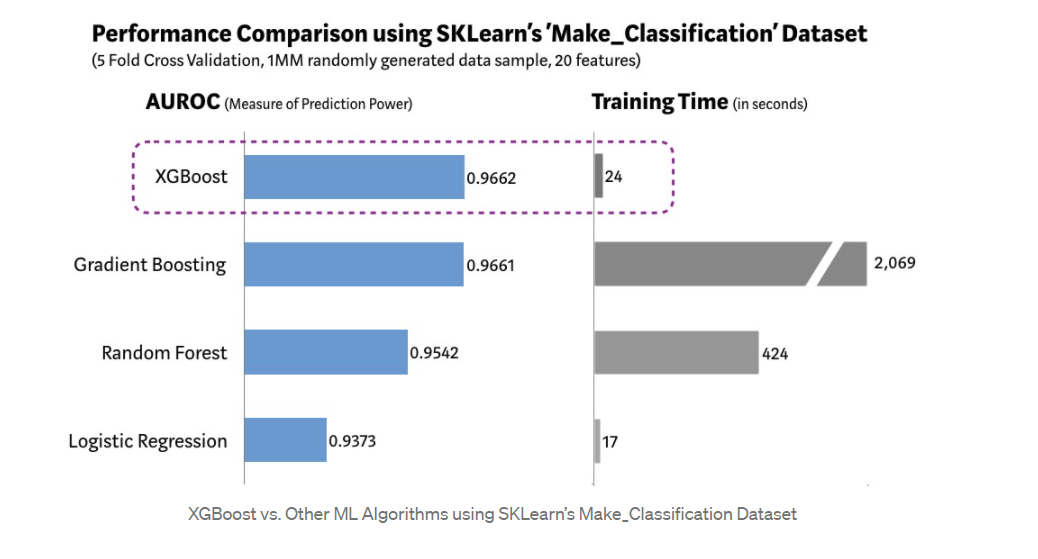
\includegraphics[width=0.75\textwidth,height=\textheight]{./Imagens/desempenho_xgboost_comparacao.png}

Dentre as leituras realizadas sobre as possibilidades de modelos e
métodos, percebemos que o XGboost tinha um ótimo desempenho comparado a
outros modelos, e que, apesar da variável \texttt{average\_rating} ser
uma variável contínua um método de classificação poderia ser adequado
para os nossos objetivos, desde que gerassemos categorias e
encaixassemos os intervalos.
\end{frame}

\hypertarget{a-inspirauxe7uxe3o-final}{%
\subsubsection{A Inspiração Final}\label{a-inspirauxe7uxe3o-final}}

\begin{frame}{A Inspiração Final}
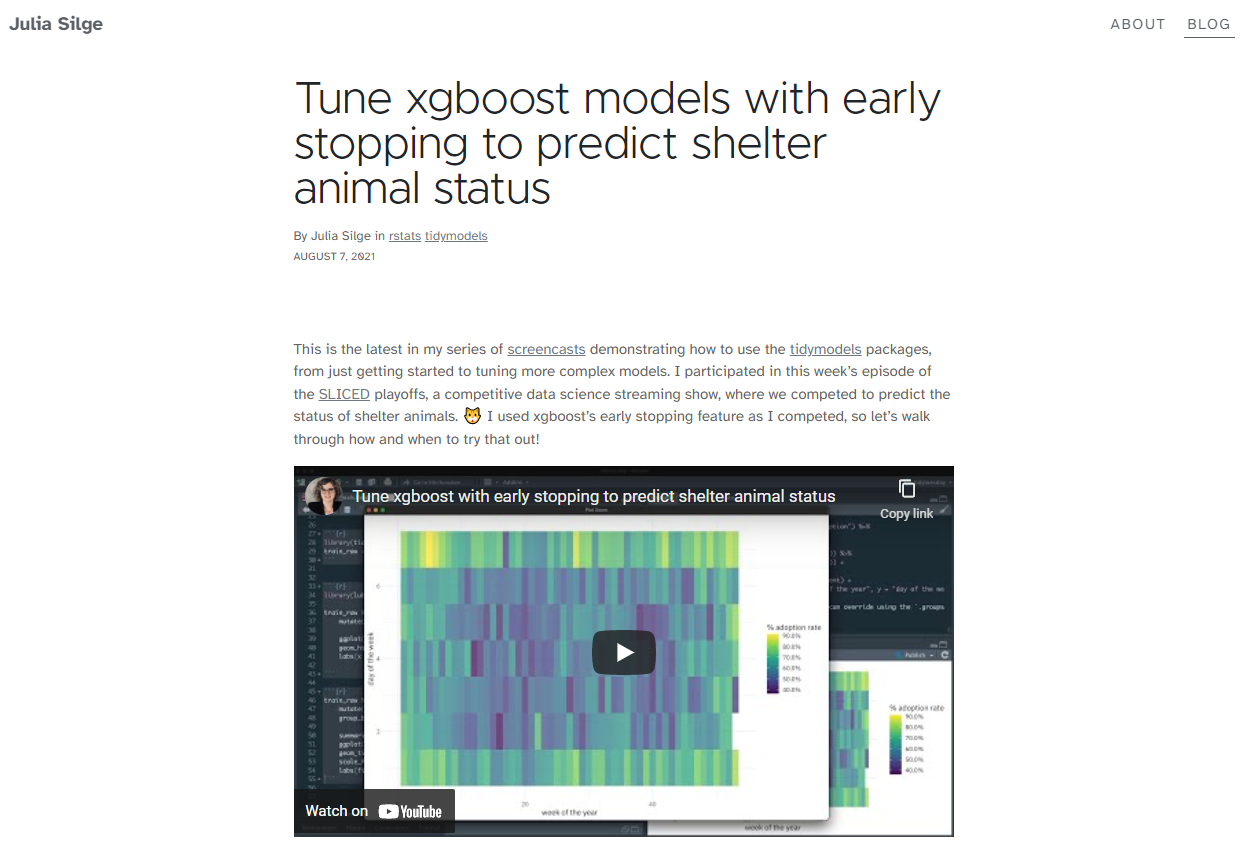
\includegraphics[width=\textwidth,height=0.9\textheight]{./Imagens/xgboost_juliasilge.png}
\end{frame}

\hypertarget{indicamos}{%
\subsubsection{Indicamos}\label{indicamos}}

\begin{frame}{Indicamos}

\includegraphics{./Imagens/juliasilge_mini.png} juliasilge.com

\begin{itemize}
\tightlist
\item
  \emph{Agora, ao nosso modelo!}
\end{itemize}
\end{frame}

\hypertarget{desenvolvimento}{%
\section{Desenvolvimento}\label{desenvolvimento}}

\hypertarget{engenharia-de-dados}{%
\subsubsection{Engenharia de Dados}\label{engenharia-de-dados}}

\begin{frame}{Engenharia de Dados}
A análise exploratória consistiu em:

\begin{itemize}
\tightlist
\item
  Limpeza dos Dados
\item
  Análise Descritiva
\end{itemize}

Dado os nossos objetivos, percebemos que algumas colunas eram
dispensáveis e outras poderiam ser transformadas, de forma que:

\begin{table}[H]
\centering
\begin{tabular}{lll}
\toprule
Excluídas & Transfomadas & Geradas\\
\midrule
bookID & average\_rating & book\_rating¹\\
title & language\_code & \\
isbn & text\_reviews\_count & prop\_text\_reviews²\\
authors & publication\_date & \\
isbn13 &  & \\
\addlinespace
publisher &  & \\
\bottomrule
\end{tabular}
\end{table}

\begin{block}{\emph{Nosso \textbf{MAIOR} desafio durante a análise e a
modelagem esteve relacionado a essa fase de engenharia de dados}}
\protect\hypertarget{nosso-maior-desafio-durante-a-anuxe1lise-e-a-modelagem-esteve-relacionado-a-essa-fase-de-engenharia-de-dados}{}
\end{block}
\end{frame}

\hypertarget{anuxe1lise-exploratuxf3ria}{%
\subsubsection{Análise Exploratória}\label{anuxe1lise-exploratuxf3ria}}

\begin{frame}[fragile]{Análise Exploratória}
\begin{itemize}
\tightlist
\item
  Para iniciar separamos o conjunto em \textbf{treino} e \textbf{teste}
  baseando-nos em 75\% das observações e balanceando-os com nossa
  variável resposta \texttt{book\_rating}.
\end{itemize}

\begin{Shaded}
\begin{Highlighting}[]
\FunctionTok{set.seed}\NormalTok{(}\DecValTok{1904}\NormalTok{, }\AttributeTok{kind =} \StringTok{"Mersenne{-}Twister"}\NormalTok{, }\AttributeTok{normal.kind =} \StringTok{"Inversion"}\NormalTok{)}
\NormalTok{livros\_split }\OtherTok{\textless{}{-}} \FunctionTok{initial\_split}\NormalTok{(livros, }\AttributeTok{prop =}\NormalTok{ .}\DecValTok{75}\NormalTok{, }\AttributeTok{strata =}\NormalTok{ book\_rating)}
\NormalTok{livros\_treino }\OtherTok{\textless{}{-}} \FunctionTok{training}\NormalTok{(livros\_split)}
\NormalTok{livros\_teste }\OtherTok{\textless{}{-}} \FunctionTok{testing}\NormalTok{(livros\_split)}
\end{Highlighting}
\end{Shaded}

\begin{itemize}
\tightlist
\item
  Em seguida verificamos a dispersão e correlação entre as variáveis
  numéricas:
\end{itemize}

\begin{Shaded}
\begin{Highlighting}[]
\FunctionTok{library}\NormalTok{(GGally)}
\end{Highlighting}
\end{Shaded}

\begin{verbatim}
## Warning: package 'GGally' was built under R version 4.0.5
\end{verbatim}

\begin{verbatim}
## Registered S3 method overwritten by 'GGally':
##   method from   
##   +.gg   ggplot2
\end{verbatim}

\begin{Shaded}
\begin{Highlighting}[]
\NormalTok{livros\_treino }\SpecialCharTok{\%\textgreater{}\%} 
  \FunctionTok{select}\NormalTok{(}\FunctionTok{where}\NormalTok{(is.numeric)) }\SpecialCharTok{\%\textgreater{}\%} 
  \FunctionTok{ggpairs}\NormalTok{(}\AttributeTok{upper =} \FunctionTok{list}\NormalTok{(}\AttributeTok{continuous =} \FunctionTok{wrap}\NormalTok{(}\StringTok{"cor"}\NormalTok{, }\AttributeTok{method =} \StringTok{"spearman"}\NormalTok{)))}
\end{Highlighting}
\end{Shaded}

\begin{verbatim}
## Warning in grid.Call(C_stringMetric, as.graphicsAnnot(x$label)): font family not
## found in Windows font database
\end{verbatim}

\begin{verbatim}
## Warning in grid.Call(C_stringMetric, as.graphicsAnnot(x$label)): font family not
## found in Windows font database
\end{verbatim}

\begin{verbatim}
## Warning in grid.Call(C_textBounds, as.graphicsAnnot(x$label), x$x, x$y, : font
## family not found in Windows font database
\end{verbatim}

\begin{verbatim}
## Warning in cor.test.default(x, y, method = method, use = use): Cannot compute
## exact p-value with ties

## Warning in cor.test.default(x, y, method = method, use = use): Cannot compute
## exact p-value with ties

## Warning in cor.test.default(x, y, method = method, use = use): Cannot compute
## exact p-value with ties

## Warning in cor.test.default(x, y, method = method, use = use): Cannot compute
## exact p-value with ties

## Warning in cor.test.default(x, y, method = method, use = use): Cannot compute
## exact p-value with ties

## Warning in cor.test.default(x, y, method = method, use = use): Cannot compute
## exact p-value with ties
\end{verbatim}

\begin{verbatim}
## Warning in grid.Call.graphics(C_text, as.graphicsAnnot(x$label), x$x, x$y, :
## font family not found in Windows font database

## Warning in grid.Call.graphics(C_text, as.graphicsAnnot(x$label), x$x, x$y, :
## font family not found in Windows font database

## Warning in grid.Call.graphics(C_text, as.graphicsAnnot(x$label), x$x, x$y, :
## font family not found in Windows font database

## Warning in grid.Call.graphics(C_text, as.graphicsAnnot(x$label), x$x, x$y, :
## font family not found in Windows font database

## Warning in grid.Call.graphics(C_text, as.graphicsAnnot(x$label), x$x, x$y, :
## font family not found in Windows font database

## Warning in grid.Call.graphics(C_text, as.graphicsAnnot(x$label), x$x, x$y, :
## font family not found in Windows font database

## Warning in grid.Call.graphics(C_text, as.graphicsAnnot(x$label), x$x, x$y, :
## font family not found in Windows font database

## Warning in grid.Call.graphics(C_text, as.graphicsAnnot(x$label), x$x, x$y, :
## font family not found in Windows font database
\end{verbatim}

\begin{verbatim}
## Warning in grid.Call(C_textBounds, as.graphicsAnnot(x$label), x$x, x$y, : font
## family not found in Windows font database
\end{verbatim}

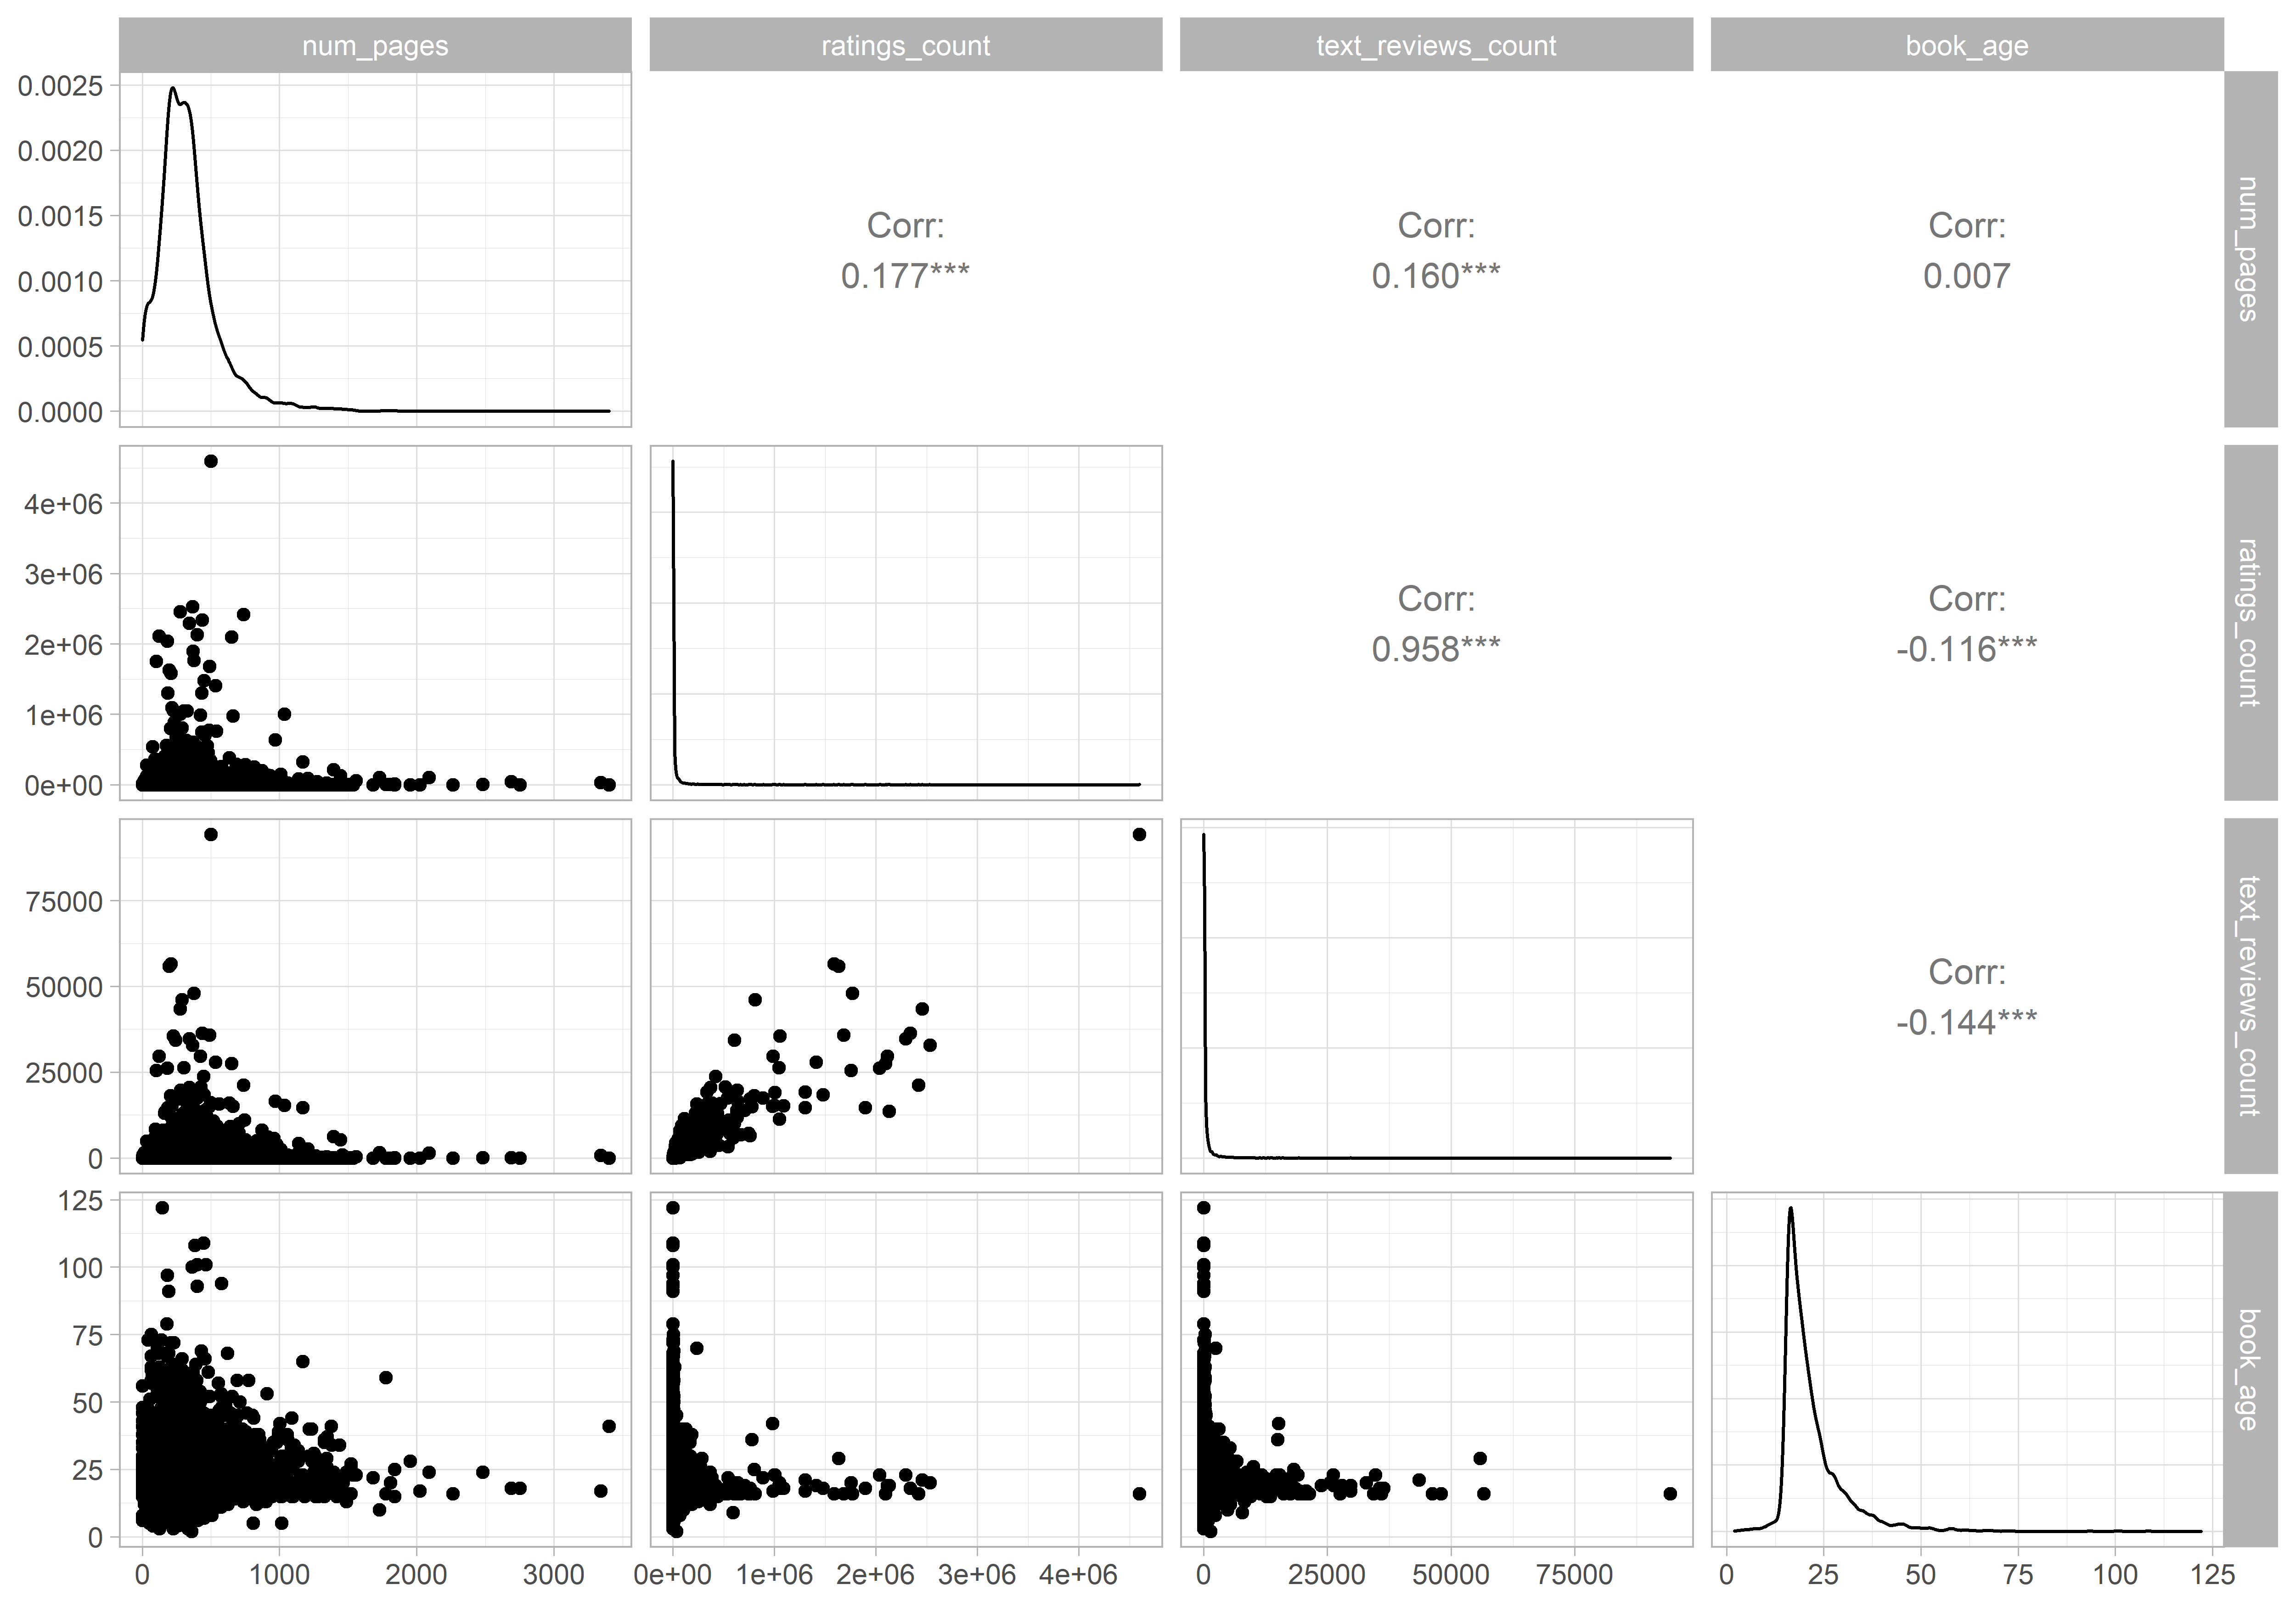
\includegraphics{apresentacao_files/figure-beamer/unnamed-chunk-4-1.png}

\begin{itemize}
\tightlist
\item
  Correlação forte entre \texttt{text\_reviews\_count} e
  \texttt{ratings\_count}.
\item
  Pensamos em gerar uma variável que considerasse a quantidade de
  \texttt{text\_reviews\_count} pois consideramos que isso seria um
  indicativo importante para nossa resposta e chegamos a uma variável
  que correspondesse a proporção entre
  \texttt{text\_reviews\_count}/\texttt{ratings\_count}
\end{itemize}

\begin{Shaded}
\begin{Highlighting}[]
\NormalTok{livros\_treino }\OtherTok{\textless{}{-}}\NormalTok{ livros\_treino }\SpecialCharTok{\%\textgreater{}\%} 
  \FunctionTok{mutate}\NormalTok{(}\AttributeTok{prop\_text\_reviews =}\NormalTok{ text\_reviews\_count }\SpecialCharTok{/}\NormalTok{ ratings\_count) }\SpecialCharTok{\%\textgreater{}\%} 
  \FunctionTok{select}\NormalTok{(}\SpecialCharTok{{-}}\NormalTok{text\_reviews\_count)}

\FunctionTok{cor}\NormalTok{(livros\_treino}\SpecialCharTok{$}\NormalTok{prop\_text\_reviews,livros\_treino}\SpecialCharTok{$}\NormalTok{ratings\_count,}
    \AttributeTok{use =} \StringTok{"complete"}\NormalTok{, }\AttributeTok{method =} \StringTok{"spearman"}\NormalTok{)}
\end{Highlighting}
\end{Shaded}

\begin{verbatim}
## [1] -0.3605444
\end{verbatim}

\begin{itemize}
\tightlist
\item
  A correlação entre \texttt{prop\_text\_reviews}e
  \texttt{ratings\_count} não indicou multirolinearidade, então
  prosseguimos com essa variável.
\end{itemize}
\end{frame}

\end{document}
